\documentclass{article}

\usepackage{graphicx,url}
\usepackage{amsfonts,amsmath,amssymb,amsthm}
\usepackage[usenames]{color}
\usepackage{courier}
\usepackage{enumerate}

\newcommand{\figref}[1]{Figure~\ref{#1}}
\newcommand{\widgraph}[2]{\includegraphics[keepaspectratio,width=#1]{#2}}
\pagestyle{empty} \addtolength{\textwidth}{1.0in}
\addtolength{\textheight}{0.5in} \addtolength{\oddsidemargin}{-0.5in}
\addtolength{\evensidemargin}{-0.5in}
\newcommand{\ruleskip}{\bigskip\hrule\bigskip}
\newcommand{\nodify}[1]{{\sc #1}} \newcommand{\points}[1]{{\textbf{[#1
points]}}}
\newcommand{\bitem}{\begin{list}{$\bullet$}%
{\setlength{\itemsep}{0pt}\setlength{\topsep}{0pt}%
\setlength{\rightmargin}{0pt}}} \newcommand{\eitem}{\end{list}}
\newcommand{\comment}[1]{}
\newcommand{\true}{\mbox{true}}
\newcommand{\Parents}{\mbox{Parents}}
\newcommand{\eat}[1]{}
\newcommand{\CInd}[3]{({#1} \perp {#2} \mid {#3})}
\newcommand{\Ind}[2]{({#1} \perp {#2})}
\setlength{\parindent}{0pt} \setlength{\parskip}{0.5ex}
\newcommand{\eparam}{\ensuremath{\eta}}
\newcommand{\meanpar}{\ensuremath{\mu}}
\newcommand{\Exs}{\ensuremath{\mathbb{E}}}
\newcommand{\bksl}{\ensuremath{\backslash}}
\newcommand{\mprob}{\ensuremath{\mathbb{P}}}
\newcommand{\indmark}{\ensuremath{\perp}}
\newcommand{\graph}{\ensuremath{G}}
\newcommand{\vertex}{\ensuremath{V}}
\newcommand{\estim}[1]{\ensuremath{\widehat{#1}}}
\newcommand{\myxsam}[1]{\ensuremath{x_{#1}}}
\newcommand{\myysam}[1]{\ensuremath{y_{#1}}}
\newcommand{\ypred}[1]{\ensuremath{\widetilde{y}^{(#1)}}}
\def\b{\backslash}
\def\child{\xi}
\newcommand{\ww}{{\bf w}}
\newcommand{\xx}{{\bf x}}
\newcommand{\yy}{{\bf y}}
\newcommand{\real}{\ensuremath{\mathbb{R}}}

\newcommand{\mbf}[1]{{\bf #1}}


%%%%%%%%%%%%%%%%%%%%%%%%%%%%%%%%%%%%%%%%%%%%%%%%%%%%%%%%%%%%%%%%%%%%

\begin{document}

\pagestyle{myheadings} \markboth{}{DS-GA-1005/CSCI-GA.2569 Problem Set 7}

{\LARGE
\begin{center}Inference and Representation, Fall 2016\end{center}
}

{\Large
Problem Set 7: Structured Prediction for Part-of-Speech Tagging
}

{\bf Due: Monday, December 5, 2016 at 3pm}  (uploaded to Gradescope/NYU Classes.)\\

{\bf Your submission should include a PDF file called ``solutions.pdf''
  with your written solutions, separate output files, and all of the
  code that you wrote.}

{\em {\bf Important:} See problem set policy on the course web site.}
\ruleskip

In this problem set, you will experiment with structured prediction using the Structured SVM algorithm on a chain-structured conditional random field (CRF). You will tackle the task of part-of-speech (POS) tagging, a problem from the natural language processing domain. POS tagging is a classification problem where the goal is to accurately predict the part of speech (e.g., noun, verb, adjective) of each word in a sentence. 

The CRF used in this prediction task is a Markov model. Let $L_i$ be the length of sentence $i$. Then, the CRF for sentence $i$ has variables $Y_1, \ldots, Y_{L_i}$, where $Y_l$ is a discrete variable denoting the part-of-speech of token $l$. The tokens are denoted by the variables $X_1, \ldots, X_{L_i}$. The CRF for a sequence of length $4$ is shown below.
\begin{center}
    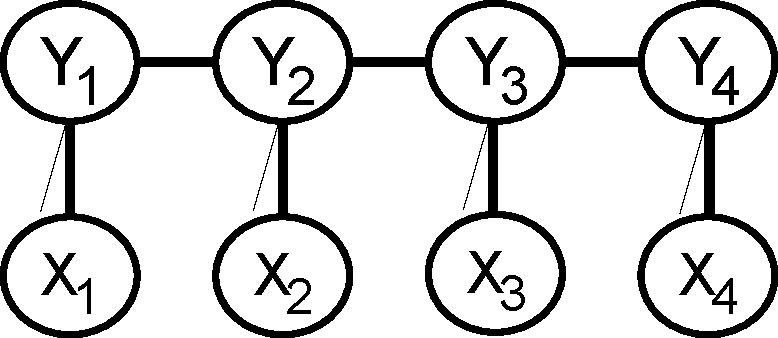
\includegraphics[scale=0.35]{crf.pdf}
\end{center}

Raw POS tagging data takes the form of a set of sentences and tag sequences. Each token (normally a word but sometimes a number or punctuation symbol) in each sentence is associated with exactly one tag. Standard POS tag sets typically include around $C=40$ distinct tags. For the purpose of this assignment, we have prepared data with a simplified tag set consisting of $C=10$ groups of tags. Each token in the data set is assigned one of these $10$ tags. To learn prediction models for the POS tagging task, we need to select a feature space to represent the tokens. For the first part of the assignment you will use simple features that we have already extracted from the tokens for you, following which you will design and implement new features.

The data consist of a set of training sentences \textit{train-i.txt} and a set of test sentences \textit{test-i.txt}. Each file contains one sentence. Each row in each file contains the raw token, the tag ID for that token, and five feature values in standard comma-separated-value (CSV) format. The format of each row is as follows: \textit{$<$Token$>$, $<$TagId$>$, $<$Bias$>$, $<$InitCap$>$, $<$AllCap$>$, $<$Pre$>$, $<$Suff$>$}. A description of the fields is given below.

\begin{center}
\begin{tabular}{|c|c|l|c|}\hline
Column  & Field  & Description               & Value\\ \hline\hline
1       & Token  &  The raw token string     & Any string\\ \hline
2       & TagID  &  The ID of the tag        & $\{1,...,10\}$\\ \hline
3       & Bias   &  Feature: Bias            & $1$\\ \hline
4       & InitCap&  Feature: Initial Capital & $\{0,1\}$\\ \hline
5       & AllCap &  Feature: All Capitals    & $\{0,1\}$\\ \hline
6       & Pre    &  Feature: Prefix ID       & $\{1,...,201\}$\\ \hline
7       & Suff   &  Feature: Suffix ID       & $\{1,...,201\}$\\ \hline
\end{tabular}
\end{center}

The $10$ tag ID's correspond to the following $10$ tag groups: verb, noun, adjective, adverb, preposition, pronoun, determiner, number, punctuation, and other. The Bias feature is a constant $1$ for all tokens. The InitCap feature is $1$ if the token string starts with a capital letter and $0$ otherwise. The AllCap feature is $1$ if the token string is all capital letters and $0$ otherwise. The Pre feature takes one of $201$ values corresponding to the most common two-character token string prefixes. The Suff feature takes one of $201$ values corresponding to the most common two-character token string suffixes.

For each word $l$ we have a feature vector $\mbf{x}_l$ of dimension $5$ (corresponding to rows 3--7 in the table), where $x_{la}$ takes values in the set $V_a$ (given in the last column of the table). 
The CRF has one parameter $w^A_{cav}$ for each of part-of-speech tag $c$, feature $a$, and feature value $v$ (note: different features $a$ have different numbers of values as given by the set $V_a$). These parameters encode the compatibility between feature values and class labels. The CRF also has one transition parameter $w^T_{cc'}$ for each pair of labels $c$ and $c'$. The transition parameters encode the compatibility between adjacent class labels in the sequence. All of the parameters can take arbitrary (positive or negative) real values. To be clear, there are exactly $(1+2+2+201+201)\cdot 10 + 10^2 = 4170$ parameters to be learned. The log-potentials are then given by:
\begin{eqnarray*}
\theta_l(y_l, \mbf{x}_l)&=& \sum_{a=1}^5 w^A_{y_l, a, x_{la}}\\
\theta_{l,l+1}(y_l, y_{l+1})&=& w^T_{y_l, y_{l+1}}
\end{eqnarray*}
Given a new sentence of length $L$, we predict its part-of-speech tagging by MAP inference in this CRF,
\[
\textrm{Predict\_POS}(\mbf{x}; \ww) = \arg\max_{{\bf y}} \sum_{l=1}^L \theta_l(y_l, {\bf x}_l) + \sum_{l=1}^{L-1}\theta_{l, l+1}(y_l, y_{l+1})
\]
Since the CRF is chain-structured, MAP inference can be performed in linear time using variable elimination or max-sum belief propagation. Suppose that ${\bf w}$ is the weight vector (i.e., of dimension 4170) and ${\bf f}(\xx, \yy)$ is the feature vector (the sufficient statistics). Then, $\textrm{Predict\_POS}(\mbf{x}; \ww) = \arg\max_{{\bf y}} \ww \cdot {\bf f}(\xx, \yy)$.

You will be using an off-the-shelf Python library {\bf PyStruct} to solve the structured SVM. The installation instructions and documentation can be found at \url{http://pystruct.github.io}

As we discussed in class, structured SVM has several advantages including a clear objective function (based on hinge loss, which is an upper bound on 0-1 loss) and max-margin regularization. 

\begin{enumerate}
\item Learn a structural SVM to model the above POS-tagging task using PyStruct. To help
you get started, we have provided you with a skeleton code \texttt{sample\_code.py} that reads
in the training data, learns a structural SVM on a subset of the training data, and performs inference on a subset of the training data. 
(For more details, refer to the code.) There
are two hyperparameters $max\_iter$ and $C$, that need to be supplied to
 \texttt{OneSlackSSVM}. For the purpose of this assignment, you can fix $max\_iter$ to $200$.
Choose $C$ using a held-out set: learn the structural SVM using the first $4500$ training samples,
and use the last $500$ training points as validate data. Let $C^*$ be the optimal
value of $C$ (giving the smallest validate error) obtained from the above process. Then, use the
entire training set to learn a model with $C=C^*$. Finally, report the test error (i.e., for the \texttt{text\_XXX.txt} files) using the learned model.

PyStruct by default uses margin scaling with Hamming loss. Its ``score'' function will report the average Hamming error (normalized by sentence length). This is the error that we want you to report in this assignment.

\item 
Repeat the experiment of question 1, but varying the number of training sentences to be the first $ 100, 200, 500$, or $1000$. The value of the hyperparameter $C$ could, in general, be different for different sizes of the training set. Hence, you should use the validate data (keep this fixed to the last 500 training points) to find the optimal value of $C$ for each size of the training data separately. Produce one plot showing both the test and train error as a function of the amount of training data (also include in the plot the result for $4500$ training sentences, as computed in the previous question).

\item For the next two questions, use the results from question 1. Out of the 10 given POS tags/classes, pick any three classes. For all ordered pairs of the three classes above, report the corresponding 
transition parameters. Comment on any interesting observations. 
For each of these three classes, which 10 features have the largest absolute value weights (i.e., contribute the most to the predictions)? You should look up the corresponding prefix and suffix IDs using the provided files \texttt{prefixes.txt} and \texttt{suffixes.txt} (do not simply report the IDs themselves, as this is not meaningful). Do the results make sense?

The learnt parameters of the model are stored in a vector \texttt{w} of the 
\texttt{OneSlackSSVM} object. 
When training a \texttt{ChainCRF} using \texttt{OneSlackSSVM} with $m$ features per training sample and $k$ classes in the directed setting, the size of weight vector \texttt{w} will be $mk + k^2$, with $mk$ features for the single-node potentials and $k^2$ features for the pairwise potentials. All the single-node features are followed by all the pairwise features. The single-node features have the following order in \texttt{w}: $m$ features for the $1^{st}$ class/POS tag (verb), $m$ features for the $2^{nd}$ class/POS tag (noun), $\ldots$. As we described earlier, the pairwise features directly give the values of the pairwise potential; the order is (class $1$, class $1$), $\ldots$, (class $1$, class $k$), $\ldots$, (class $k$, class $1$), $\ldots$, (class $k$, class $k$).
Thus, for our problem setting, the last 100 values of the vector correspond to the 
transition parameters.

\item Choose any 10 test sentences and, using the \texttt{predict} function of 
\texttt{OneSlackSSVM}, find the POS tags assigned by the model to the words in the
sentences. Compare the predicted tags with the actual tags, and report any mismatches.

\end{enumerate}

{\em Acknowledgement:} This problem set is partly based on an assignment developed at UMass Amherst by Ben Marlin, Andrew McCallum, Sameer Singh and Michael Wick.\\

\bibliographystyle{plain}
\bibliography{refs}

%%%%%%%%%%%%%%%%%%%%%%%%%%%%%%%%%%%%%%%%%%%%%%%%%%%%%%%%%%%%%%%%%%%%%%%%%%

\end{document}

